% Options for packages loaded elsewhere
\PassOptionsToPackage{unicode}{hyperref}
\PassOptionsToPackage{hyphens}{url}
\PassOptionsToPackage{dvipsnames,svgnames,x11names}{xcolor}
%
\documentclass[
  11pt,
]{article}
\usepackage{amsmath,amssymb}
\usepackage[]{mathpazo}
\usepackage{iftex}
\ifPDFTeX
  \usepackage[T1]{fontenc}
  \usepackage[utf8]{inputenc}
  \usepackage{textcomp} % provide euro and other symbols
\else % if luatex or xetex
  \usepackage{unicode-math}
  \defaultfontfeatures{Scale=MatchLowercase}
  \defaultfontfeatures[\rmfamily]{Ligatures=TeX,Scale=1}
\fi
% Use upquote if available, for straight quotes in verbatim environments
\IfFileExists{upquote.sty}{\usepackage{upquote}}{}
\IfFileExists{microtype.sty}{% use microtype if available
  \usepackage[]{microtype}
  \UseMicrotypeSet[protrusion]{basicmath} % disable protrusion for tt fonts
}{}
\makeatletter
\@ifundefined{KOMAClassName}{% if non-KOMA class
  \IfFileExists{parskip.sty}{%
    \usepackage{parskip}
  }{% else
    \setlength{\parindent}{0pt}
    \setlength{\parskip}{6pt plus 2pt minus 1pt}}
}{% if KOMA class
  \KOMAoptions{parskip=half}}
\makeatother
\usepackage{xcolor}
\usepackage[margin = 1in]{geometry}
\usepackage{graphicx}
\makeatletter
\def\maxwidth{\ifdim\Gin@nat@width>\linewidth\linewidth\else\Gin@nat@width\fi}
\def\maxheight{\ifdim\Gin@nat@height>\textheight\textheight\else\Gin@nat@height\fi}
\makeatother
% Scale images if necessary, so that they will not overflow the page
% margins by default, and it is still possible to overwrite the defaults
% using explicit options in \includegraphics[width, height, ...]{}
\setkeys{Gin}{width=\maxwidth,height=\maxheight,keepaspectratio}
% Set default figure placement to htbp
\makeatletter
\def\fps@figure{htbp}
\makeatother
\setlength{\emergencystretch}{3em} % prevent overfull lines
\providecommand{\tightlist}{%
  \setlength{\itemsep}{0pt}\setlength{\parskip}{0pt}}
\setcounter{secnumdepth}{-\maxdimen} % remove section numbering
\newlength{\cslhangindent}
\setlength{\cslhangindent}{1.5em}
\newlength{\csllabelwidth}
\setlength{\csllabelwidth}{3em}
\newlength{\cslentryspacingunit} % times entry-spacing
\setlength{\cslentryspacingunit}{\parskip}
\newenvironment{CSLReferences}[2] % #1 hanging-ident, #2 entry spacing
 {% don't indent paragraphs
  \setlength{\parindent}{0pt}
  % turn on hanging indent if param 1 is 1
  \ifodd #1
  \let\oldpar\par
  \def\par{\hangindent=\cslhangindent\oldpar}
  \fi
  % set entry spacing
  \setlength{\parskip}{#2\cslentryspacingunit}
 }%
 {}
\usepackage{calc}
\newcommand{\CSLBlock}[1]{#1\hfill\break}
\newcommand{\CSLLeftMargin}[1]{\parbox[t]{\csllabelwidth}{#1}}
\newcommand{\CSLRightInline}[1]{\parbox[t]{\linewidth - \csllabelwidth}{#1}\break}
\newcommand{\CSLIndent}[1]{\hspace{\cslhangindent}#1}
\usepackage{setspace}\doublespacing
\usepackage[utf8]{inputenc}
\usepackage[T1]{fontenc}
\usepackage{booktabs}
\usepackage{longtable}
\usepackage{array}
\usepackage{multirow}
\usepackage{wrapfig}
\usepackage{float}
\usepackage{colortbl}
\usepackage{pdflscape}
\usepackage{tabu}
\usepackage{threeparttable}
\usepackage{threeparttablex}
\usepackage[normalem]{ulem}
\usepackage{makecell}
\usepackage{xcolor}
\ifLuaTeX
  \usepackage{selnolig}  % disable illegal ligatures
\fi
\IfFileExists{bookmark.sty}{\usepackage{bookmark}}{\usepackage{hyperref}}
\IfFileExists{xurl.sty}{\usepackage{xurl}}{} % add URL line breaks if available
\urlstyle{same} % disable monospaced font for URLs
\hypersetup{
  pdftitle={Dynamic Prediction of Non-Guassian Outcome with fast Generalized Functional Principal Analysis},
  pdfauthor={Ying Jin; Andrew Leroux},
  colorlinks=true,
  linkcolor={blue},
  filecolor={Maroon},
  citecolor={Blue},
  urlcolor={Blue},
  pdfcreator={LaTeX via pandoc}}

\title{Dynamic Prediction of Non-Guassian Outcome with fast Generalized
Functional Principal Analysis}
\author{Ying Jin \and Andrew Leroux}
\date{April 06, 2023}

\begin{document}
\maketitle

\hypertarget{introduction}{%
\section{Introduction}\label{introduction}}

Biomedical investigators are often interested in predicting future
observations of subjects based on their historical data, typically
referred to as dynamic prediction. Traditionally, this type of data has
been modeled either marginally, such as generalized estimating
equations, or conditionally on specific subjects, such as mixed effect
models (\protect\hyperlink{ref-Laird1982}{Laird and Ware 1982};
\protect\hyperlink{ref-liang1986}{LIANG and ZEGER 1986};
\protect\hyperlink{ref-lindstrom1990}{Lindstrom and Bates 1990};
\protect\hyperlink{ref-davidian2003}{{``Nonlinear models for repeated
measurement data''} 2003}). For subject-specific models, predictions are
made based on the correlation between repeated measures from the same
subject and covariates that can be either fixed or varying. Software and
methods for dynamic prediction have been developed for Gaussian
{[}leroux2016; Shang (\protect\hyperlink{ref-shang2017}{2017}); Goldberg
et al. (\protect\hyperlink{ref-goldberg2014}{2014}){]}, non-Gaussian
data (\protect\hyperlink{ref-chiou2012}{Chiou 2012};
\protect\hyperlink{ref-GLMMadaptive}{Rizopoulos 2022}), and
time-to-event outcomes (\protect\hyperlink{ref-jmbook}{Rizopoulos 2012};
\protect\hyperlink{ref-suresh2017}{Suresh et al. 2017}). However, with
the notable exception of Leroux et al.
(\protect\hyperlink{ref-leroux2016}{2018a}), existing methods are either
limited in their flexibility (both fixed and random effect structure,
e.g.~random slope and intercept), computationally unfeasible for large
datasets, or both. These issues are particularly acute for data which
are measured densely, as is often the case with functional data, or when
data are non-Gaussian.

While methods with accompanying software for modeling complex functional
data with non-linear fixed and random effects exist for both Gaussian
and non-Gaussian data, software is largely limited to the refund package
in the statistical software R
(\protect\hyperlink{ref-Scheipl2014}{Scheipl et al. 2014};
\protect\hyperlink{ref-wood2014}{Wood and Scheipl 2014};
\protect\hyperlink{ref-refundpkg}{\textbf{refundpkg?}}). However, these
methods and software implementations do not currently allow for dynamic
prediction. In addition to the methods implemented in the refund
package, other work has been done on the fitting of functional
regression models to non-Gaussian functional data. For example, Chen et
al. (\protect\hyperlink{ref-chen2013}{2013}) proposed approaches to fit
marginal functional models that is compatible to multi-level,
generalized outcomes. Goldsmith et al.
(\protect\hyperlink{ref-goldsmith2015}{2015}) established a model
framework that takes into account the fixed effect of time-invariant
covariates, with parameters estimated with Bayesian method in
\emph{Stan}. Gertheiss et al.
(\protect\hyperlink{ref-gertheiss2016}{2016}) identified bias introduced
by directly applying FPCA methods to generalized functions, and proposed
to address this problem using a two-stage joint estimation strategy.
Linde (\protect\hyperlink{ref-linde2019}{2009}) used an adapted Bayesian
variational algorithm for FPCA of binary and count data. In terms of
implementation, Wrobel et al. (\protect\hyperlink{ref-wrobel2019}{2019})
proposed a fast, efficient way to fit GFPCA on binary data using EM
algorithm, accompanied by the an open source R package \emph{registr}.

Existing research on dynamic prediction with functional data has focused
primarily on continuous/Gaussian outcomes, usually modelling
subject-specific random effects with FPCA
(\protect\hyperlink{ref-chiou2012}{Chiou 2012};
\protect\hyperlink{ref-goldberg2014}{Goldberg et al. 2014};
\protect\hyperlink{ref-shang2017}{Shang 2017}). Kraus
(\protect\hyperlink{ref-kraus2015}{2015}) has used this approach to
predict missing observations in partially observed function tracks, and
Delaigle and Hall (\protect\hyperlink{ref-delaigo2016}{2016}) achieved
similar goals using Markov Chains. While methods mentioned above used
only partial observations for prediction with an intercept-only model,
Leroux et al. (\protect\hyperlink{ref-leroux2016}{2018a}) proposed
Functional Concurrent Regression (FCR) framework which can incorporate
the effect of subject-specific predictors. Although methodological
development exists, flexible software for implementing these methods is
still relatively sparse with the exception of the fcr
(\protect\hyperlink{ref-fcrpkg}{\textbf{fcrpkg?}}) package accompanying
(\protect\hyperlink{ref-leroux2016}{Leroux et al. 2018a}).

In this paper, we aim to develop a fast, scalable method for dynamic
prediction of generalized functional outcomes using the principals of
local generalized linear mixed effects models combined with functional
principal components analysis of the estimated latent processes. The
proposed method is designed to handle dense, regularly measured
functional data and is extremely computationally efficient relative to
the model complexity. Section 2 explains the implementation procedure of
the proposed method. In Section 3, we illustrate the performance and
efficiency of our proposed method in a simulation study. In Section 4,
we apply this method to a real world dataset from a weight loss study.
Section 5 presents a discussion of advantages and limitation of the
proposed method.

\hypertarget{method}{%
\section{Method}\label{method}}

The observed data for a single subject \(i\) is (\(t\), \(Y_i(t)\)),
where \(t\) consists of dense, discrete points along the domain of data
collection. In practice, \(t\) is usually a time index along the
duration of study. We hereafter refer to the range of \(t\) as the
``functional domain''. For simplicity, we further assume that outcomes
are collected on a regular grid over the functional domain, meaning that
\(t\) are evenly distributed and does not change across subjects.

\(Y_i(t)\) is the non-Gaussian outcome observed at \(t\). We assume that
the outcome \(Y_i(t)\) can be characterized by a latent continuous
function \(\eta_i(t)\). That is, at a specific t, \(Y_i(t)\) follows a
exponential family distribution such that:

\[
g[E(Y_i(t))] = \eta_i(t) = \beta_0(t)+b_i(t)
\]

where g is an appropriate link function, \(\beta_0(t)\) is the
population mean of latent function, and \(b_i(t)\) is a subjects-level
random effect function following a zero-mean Gaussian process with
covariance operator \(\Sigma_b\). By the Karhunen-Loève theorem,
\(b_i(t)\) can be represented as the linear combination of a infinite
set of orthogonal functions:
\(b_i(t)=\sum_{k=1}^{\infty}\xi_{ik}\phi_{k}(t)\). In practice,
\(b_i(t)\) is approximated using a finite \(K\) number of basis
functions.

Estimation of \(b_i(t)\) involves estimating both
\(\{\phi_k(t): t \in \cal{T}, 1 \leq k \leq K\}\) and
\(\{\xi_{ik}: 1 \leq i \leq N, 1 \leq k \leq K\}\). For Gaussian data
this may be done by directly estimating the covariance operator
\(\Sigma_b\) using either method of moments (if the data are relatively
small) or using faster methods such as the FACE method {[}reference -
FACE{]}. However, for non-Gaussian data, direct estimation is not
possible. Instead, one may choose to estimate \(b_i(t)\) first using a
flexible spline basis (e.g.~B-splines) with dimension \(K^b\) such that
\(K^B > K\), assuming an unstructured correlation between
subject-specific spline coefficients, then orthogonalizing the resulting
estimates via eigendecomposition or singular value decomposition. This
general approach forms the basis for estimation for several GFPCA
methods {[}references - goldsmith, julia's EM algorithm{]}. However,
this approach results in rapidly escalating computational burden as both
the number of subjects, \(N\), and the density of the observed
functional predictor increases. Note that if the covariance operator
\(\Sigma_b\) is relatively complex, then \(K\) may be large and not well
approximated using simple basis functions, \(\phi_k\) (e.g.~random
intercept and slope).

Beyond the computational burden associated with fitting the model of
interest, for dynamic prediction one must then estimate the scores for a
new subject \(u\) not used in model fitting. Typically this takes the
form of the conditional expectation of the scores
\(E[\xi_{uk}|\bf{\Theta}, \bf{y}_{u}]\) where \(\bf{\Theta}\) represents
the set of parameters estimated by the model (i.e.~parameters associated
with \(\beta_0(t), \Sigma_b\)) and \(\bf{y}_u\) are the non-Gaussian
data for the new subject. Estimation of the random effects for a new
subject is non-trivial and not implemented for even very simple models
in most random effects software packages such as lme4 {[}reference{]}
and nlme {[}reference{]}. Our proposed method bypasses this problem by
using local generalized linear mixed models to estimate the covariance
operator \(\Sigma_b\) directly on the latent scale, then using the
closed form solution for the best linear unbiased predictor of Gaussian
random effects. Estimation is made fast for even very large data through
the use of the FACE methodology for FPCA on the latent estimates
obtained from local models. Because the local models are very simple
GLMMs, estimation is also fast for the local models.

\textbf{Fast Generalized FPCA} Based on the problem set up above, we
propose the following algorithm for fast, generalizable implementation
of FPCA (fGFPCA) on the unobserved latent process \(\eta_i(t)\):

\begin{enumerate}
\def\labelenumi{\arabic{enumi}.}
\item
  Bin the observed outcomes in to small, non-overlapping, equal length
  intervals. We hereafter index the bins by their midpoints \(s\). The
  number of observations from the same subject in bin \(s\) is \(n_s\),
  and \(t_{sj}\) refers to the jth observation point in bin \(s\).
\item
  Fit a local Generalized Mixed Model at every bin. Specifically, at bin
  \(s\), we fit \(g[E(Y_i(t_{sj}))] = \beta_0(s)+b_i(s)\),
  \(j\in\{1, ..., n_s\}\). From this series of models we can estimate
  the individual latent functions at every bin:
  \(\hat{\eta}_i(s) = \hat{\beta}_0(s)+\hat{b}_i(s)\).
\item
  Fit FPCA on the estimated latent functions:
  \(\hat{\eta}_i(s) = f_0(s)+\sum_{k=1}^K\xi_{ik}\phi_{k}(s)+\epsilon_i(s)\),
  and obtain estimates of basis functions
  \(\boldsymbol{\Phi} = \{\phi_1(s), ...,\phi_k(s)\}\), eigenvalues
  \(\hat{\lambda}_1...\hat{\lambda}_k\), mean function \(\hat{f}_0(s)\)
  and residual variance \(\hat{\sigma}^2\).
\end{enumerate}

\textbf{Ying, include the formulas for your conditional expectation here
to obtain random effects estimates }

\textbf{Dynamic prediction} Now assume we have a new observations with
partially observed outcome \(Y_{new}(t)\), \(t\leq t_m\). The maximum
observed point is \(t_m\), which is a point along the functional domain
and belongs to bin \(s_m\) on the binned grid from step 1 above. With
components extracted from the FPCA model in step 3, we will be able to
make predictions on the future, unobserved bins. Specifically, with the
partially observed binary function \(Y_{new}(t)\), we will be able to
calculate the maximum likelihood estimate (MLE) of the subject-specific
PC scores \(\hat{\xi}_{ik}\). Then the value of latent functions at
unobserved points can be estimated as
\(\hat{\eta_i}(s)=\hat{f}_0(s)+\sum_{k=1}^K\hat{\xi}_{ik}{\phi}_k(s)\)

Following the algorithm above, predictions of individual latent
functions are made on the binned grid based on partially observed tracks
on the un-binned grid. Since the bins are set up to be small in length,
the binned grid would still be dense. However, in situations where
predictions on the original, un-binned grid is needed, linear
interpolation of estimated latent function tracks turns out to be a
fast, convenient way with good performance for prediction at points
between bins.

\hypertarget{simulation}{%
\section{Simulation}\label{simulation}}

In this section, we illustrate the predictive performance and
computational efficiency of the proposed method through a simulation
study. We simulated 50 datasets, each with 500 subjects. For every
subject, we generate 1000 binary outcomes \(Y_i(t) \in \{0, 1\}\) across
functional domain \(t \in (0, 1000]\), where the distribution of outcome
is characterized by a continuous latent function. The data generation
mechanism can be expressed as follows:

\[\begin{aligned}
Y_i(t) & \sim Binomial(\frac{exp(\eta_i(t))}{1+exp(\eta_i(t))}) \\
\eta_i(t) &= f_0(t)+ \xi_{i1}\sqrt{2}sin(2\pi t)+\xi_{i2}\sqrt{2}cos(2\pi t)+\xi_{i3}\sqrt{2}sin(4\pi t)+\xi_{i4}\sqrt{2}cos(4\pi t)
\end{aligned}\]

In this simulation, we set \(f_0(t) = 0\). \(\xi_{ik}\) are mutually
independent normal random variables \(\xi_{ik}\sim N(0, \lambda_k)\).
Here we set the values of \(\lambda_k\) to be \(0.5^{k-1}\),
\(k \in (1,..., 4)\). In addition, for simplicity of presentation, we
generate data on a regular grid, which means observations points are
equally distributed across \((0, 1000]\) and are the same for all
subjects.

We use two metrics to evaluate the out-of-sample predictive performance:
integrated squared error (ISE) and
Area-Under-the-Receiver-Operator-Curve (AUC). ISE assesses the
prediction accuracy of latent continuous functions. It is evaluated on
the binned grid at midpoints of each unobserved bin. With observations
up to bin \(s_m\), ISE is defined as
\(\frac{1}{N}\sum_{i=1}^N\sum_{s>s_m} (\hat{\eta}_i(s)-\eta_i(s))^2\).
The second metric, AUC, focuses on evaluation of prediction of the
binary outcome. Since the binary outcomes are generated on the original,
un-binned grid, we evaluated AUC on this grid by estimating values of
latent functions between bins with linear interpolation.

As a reference method, we compare our method to Generalized Linear Mixed
Models using Adaptive Gaussian Quadrature (GLMMadaptive). This is one of
the fastest existing method developed for dynamic prediction of repeated
generalized outcomes. Just like many mixed models, this method is very
limited in terms of flexibility if one wishes to obtain estimates in a
reasonable time frame. For example, the model used for prediction of our
simulated datset would simply be an linear model with one covariate
indicating observation time:
\(g(E(Y_i)) = \beta_0+\beta_1t+b_{i0}+b_{i1}t\). While the flexibility
of this mixed model can be increased using spline functions, the
dimension of spline basis is also restricted by computational ability,
and is unfeasible to implement under the scale of our simulated data or
the complexity of our proposed method.

The average ISE and AUC across all simulation is presented in Table 1,
and Figure 1 presents the predicted latent function of four randomly
selected subjects from the first simulated dataset. The prediction is
made conditioning on different length of observed track (specifically,
with observations up to t = 200, 400, 600, 800 respectively), and
evaluation is made on equal-length time windows on the unobserved tracks
following the maximum observation time. As Table 1 reveals, the proposed
method (fGFPCA) outperforms GLMMadaptive under every scenario, which was
expected since the linear model structure of GLMM is too simple for the
cyclic data generation mechanism. In addition, fGFPCA also took less
computation time. For one simulated dataset, fGFPCA spent 4.94 minutes
on model fitting and out-of-sample prediction overall, while
GLMMadaptive took 5.11 minutes.

Because of the flexibility of our proposed model framework, the accuracy
of prediction at specific time points would improve as more observed
data is collected. This is revealed in Table 1 as ISE decreases and AUC
increases with maximum observed time (left-to-right), also in Figure 1
as predicted curves get closer to the true latent function with longer
observed track. However the same tendency is not observed with
GLMMadaptive models, as a result of restricted model flexibility. A
linear model that fits well to a specific part can fit very badly to
other parts along the underlying latent function tracks, especially when
the shapes of functions are wiggly or cyclic. Therefore, more
observations do not necessarily make the model more predictive.

\begin{figure}
\centering
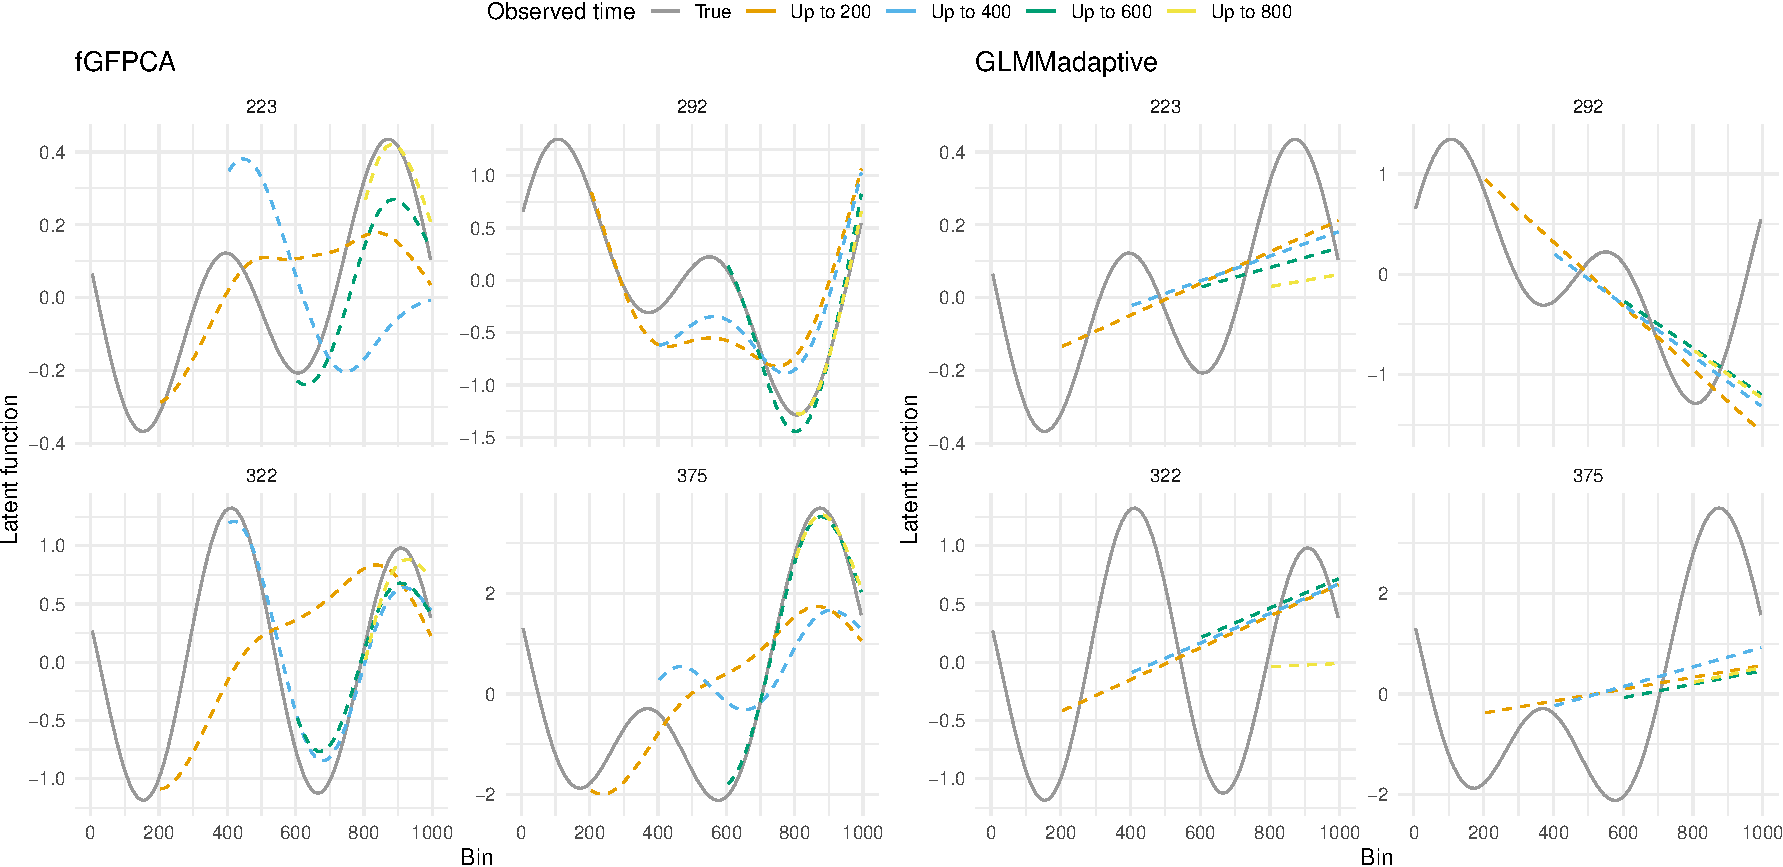
\includegraphics{Manuscript_edit_files/figure-latex/Figure-1.pdf}
\caption{Predicted track of four randomly selected subjects from one
simulated dataset. The grey solid line indicates the true latent
continuous function. The dashed lines indicated predicted latent
function tracks, and color indicates different observation time.}
\end{figure}

\begin{table}

\caption{\label{tab:format table}Predictive performance of fGFPCA and GLMM adaptive on the simulated datasets. ISE and AUC are average values across all 50 simulations.}
\centering
\begin{tabular}[t]{llccccccc}
\toprule
\multicolumn{1}{c}{ } & \multicolumn{8}{c}{Maximum observed time} \\
\cmidrule(l{3pt}r{3pt}){2-9}
\multicolumn{1}{c}{ } & \multicolumn{4}{c}{fGFPCA} & \multicolumn{4}{c}{GLMMadaptive} \\
\cmidrule(l{3pt}r{3pt}){2-5} \cmidrule(l{3pt}r{3pt}){6-9}
  & 200 & 400 & 600 & 800 & 200 & 400 & 600 & 800\\
\midrule
\addlinespace[0.3em]
\multicolumn{9}{l}{\textbf{Prediction time window}}\\
\addlinespace[0.3em]
\multicolumn{9}{l}{\textbf{ISE}}\\
\hspace{1em}\hspace{1em}(200, 400] & 15.29 &  &  &  & 38.20 &  &  & \\
\hspace{1em}\hspace{1em}(400, 600] & 18.68 & 8.53 &  &  & 28.59 & 26.46 &  & \\
\hspace{1em}\hspace{1em}(600, 800] & 22.53 & 5.51 & 1.65 &  & 31.32 & 27.97 & 27.40 & \\
\hspace{1em}\hspace{1em}(800, 1000] & 11.34 & 8.72 & 1.90 & 1.30 & 55.19 & 46.89 & 58.57 & 59.25\\
\addlinespace[0.3em]
\multicolumn{9}{l}{\textbf{AUC}}\\
\hspace{1em}\hspace{1em}(200, 400] & 0.74 &  &  &  & 0.59 &  &  & \\
\hspace{1em}\hspace{1em}(400, 600] & 0.66 & 0.73 &  &  & 0.52 & 0.59 &  & \\
\hspace{1em}\hspace{1em}(600, 800] & 0.71 & 0.79 & 0.80 &  & 0.67 & 0.70 & 0.69 & \\
\hspace{1em}\hspace{1em}(800, 1000] & 0.74 & 0.75 & 0.78 & 0.78 & 0.52 & 0.56 & 0.53 & 0.57\\
\bottomrule
\end{tabular}
\end{table}

\hypertarget{data-application}{%
\section{Data application}\label{data-application}}

In this section, we illustrate the performance of our proposed method
using data from a randomized trial on weight loss at University of
Colorado Anschutz Medical Campus
(\protect\hyperlink{ref-bothwell2022}{Bothwell et al. 2022};
\protect\hyperlink{ref-ostendorf2022}{Ostendorf et al. 2022}). The study
originally aimed to study the effect of dietary strategies on weight
loss, and participants were given a smart scale for daily at-home
weighing. This record was then scaled into a binary indicator of
participant adherence to the daily-weigh-in procedure, where 1 indicates
participants followed the requirement and 0 otherwise. In this section,
we will use this series of daily indicators as the binary functional
outcome, and use the proposed method to dynamically predict participant
adherence on future days given historical track.

The dataset includes 55 participants aged 22-56 at baseline. Adherence
to daily weigh-in is available along 400 consecutive days for all
participants. In other words, for each individual, 400 binary
measurements were taken on a regular grid along the functional domain
(number of days into the study). We will fit both fGFPCA and
GLMMadaptive models and compared their performance on this data. For
fGFPCA, every 10 observations are binned together, resulting in 40 bins
for final model fitting. Linear interpolation was used for extension
from the binned grid back to the un-binned grid. Since the latent
continuous function tracks are not known in this case, prediction
performance on evaluated with AUC alone.

Table 2 compares the predictive performance of both models. Similar to
the simulatio study, prediction is made conditioning on observations up
to the 100th, 200th and 300th day respectively, and evaluation is made
every 100 days following the maximum observation time. As is revealed,
when the observed time is short (up to 100th day), the two method
performed similarly when predicting recent days, however fGFPCA did
better in predicting further days along the trial (prediction time
window of \((300, 400]\)). As more observations coming in, fGFPCA sees
increasingly higher AUC compared to GLMMadaptive model. This could be a
result of the difference in model flexibility of the two methods. While
the linear relationship in underlying latent functions are not likely to
change immediately following the observed track, the whole track could
be much more complex. Therefore, while fGFPCA performs similarly to
GLMMadaptive right after the end of observation, it does a much better
job capturing the underlying pattern along the whole track. Figure 2
further illustrate such difference using predicted latent function
tracks of four randomly drawn subjects.

\begin{figure}
\centering
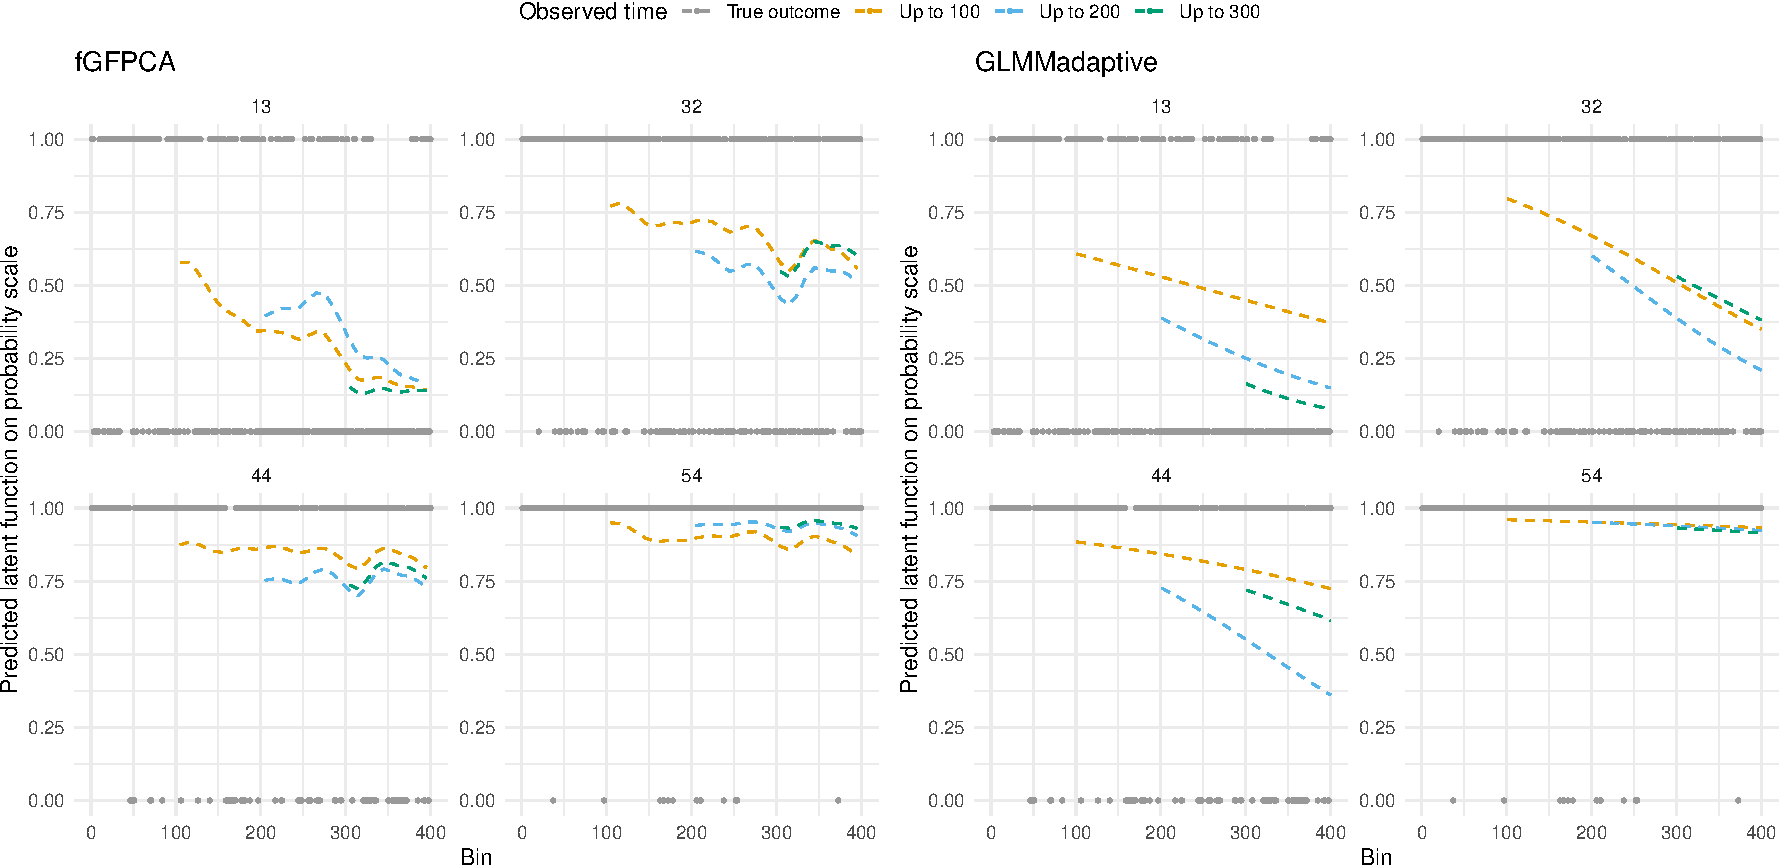
\includegraphics{Manuscript_edit_files/figure-latex/Figure_appl-1.pdf}
\caption{Predicted track of four randomly selected subjects from the
daily weigh-in dataset. The grey solid line indicates the true latent
continuous function. The dashed lines indicated predicted latent
function tracks, and color indicates different observation time.}
\end{figure}

\begin{table}

\caption{\label{tab:unnamed-chunk-3}AUC of fGFPCA and GLMM adaptive on the daily weigh-in dataset}
\centering
\begin{tabular}[t]{llccccc}
\toprule
\multicolumn{1}{c}{ } & \multicolumn{6}{c}{Maximum observed time} \\
\cmidrule(l{3pt}r{3pt}){2-7}
\multicolumn{1}{c}{ } & \multicolumn{3}{c}{fGFPCA} & \multicolumn{3}{c}{GLMMadaptive} \\
\cmidrule(l{3pt}r{3pt}){2-4} \cmidrule(l{3pt}r{3pt}){5-7}
  & 100 & 200 & 300 & 100 & 200 & 300\\
\midrule
\addlinespace[0.3em]
\multicolumn{7}{l}{\textbf{Prediction time window}}\\
\hspace{1em}(100, 200] & 0.75 &  &  & 0.76 &  & \\
\hspace{1em}(200, 300] & 0.77 & 0.82 &  & 0.76 & 0.80 & \\
\hspace{1em}(300, 400] & 0.76 & 0.81 & 0.84 & 0.74 & 0.78 & 0.82\\
\bottomrule
\end{tabular}
\end{table}

\hypertarget{discussion}{%
\section{Discussion}\label{discussion}}

The simulation study and data application above have illustrated the
feasibility and utility of the proposed method, even for large datasets
and complex latent processes/random effect structures. can achieve
better predictive performance with much less computational burden.
Compared to competing methods, fGFPCA can accommodate extremely flexible
correlation structure between repeated measure, which is particularly
useful when outcome is generated from latent functions with highly
non-linear patterns. Due to the comparative flexibility of the fGFPCA
approach, fGFPCA has much lower ISE and higher AUC than GLMM. As
expected, the dynamic prediction accuracy of fGFPCA improves as more
data are availble for predictions. Moreover, fGFPCA also significantly
reduce time spent on both model fitting and prediction, allowing for
scaling of models and predictions which are infeasible with existing
approaches. In fact, as far as we are aware of, the proposed method is
the only feasible method that can handle the scale of the simulated
datasets with compatible flexibility.

\textbf{Andrew: I would delete this paragraph, honestly}

While the proposed method achieved good accuracy of point prediction, it
is more complicated to develop a straightforward, interpretable metric
to evaluate the precision of prediction. The challenge arises from the
fact that fitting local GLMMs (Step 2) and FPCA (Step 3) can both
introduce uncertainty to the final prediction. Since they are
implemented consecutively, it is not clear how the uncertainty from both
procedures should be integrated into one single interval estimator. In
practice, one could consider developing interval predictions conditional
on the local GLMMs, quantifying uncertainty of individual score
estimates from FPCA model alone. Since the score \(\hat{\xi}_{ik}\) is
essentially a maximum likelihood estimate, it is natural to estimate its
variance based on likelihood theory with observed information
\({I}(\hat{\xi}_{ik})\). Therefore, the variation of prediction interval
is:

\[Var(\hat{\eta_i}(s)-\eta_i(s))=\boldsymbol{\Phi}(s)I(\hat{\boldsymbol{\xi}}_i)\boldsymbol{\Phi}^T(s)+\hat{\sigma_{\epsilon}}^2\]
Where \(\boldsymbol{\Phi}(s)=(\phi_1(s)...\phi_K(s))\) and
\(\hat{\boldsymbol{\xi}}_i=(\hat{\xi}_{i1}, ...,\hat{\xi}_{iK})\).

A few open questions remain with the fGFPCA approach. The choices
involved in the binning procedure in Step 1 can also affect the final
predictive performance, thus further investigations are needed to
quantify such effects. Predictive accuracy and computational speed can
change with bin width, number of observations in each bin, whether the
bins overlap with each other, also whether the bins are equally spaced
along the functional grid. Moreover, if the bins are very narrow with
only a few observations, local models may be non-identifiabile,
resulting in bins with no point estimates. While this may not overly
impact point final predictions, it is currently unclear as to when this
issue warrants concern. In practice, we expect this to happen when the
measurements are sparse or sample size is small. However, the
methodology here is designed for large, dense functional data and thus
not currently appropriate in such scenarios. In this case, existing
methods may be sufficiently flexible and computationally feasible.

\hypertarget{references}{%
\section{References}\label{references}}

\hypertarget{refs}{}
\begin{CSLReferences}{1}{0}
\leavevmode\vadjust pre{\hypertarget{ref-bothwell2022}{}}%
Bothwell, S., Kaizer, A., Catenacci, V., and Wrobel, J. (2022),
{``Pattern-based clustering of daily weigh-in trajectories using dynamic
time warping,''} \emph{Biometrics}.
\url{https://doi.org/10.1111/biom.13773}.

\leavevmode\vadjust pre{\hypertarget{ref-chen2013}{}}%
Chen, H., Wang, Y., Paik, M. cho, and Choi, H. A. (2013), {``A marginal
approach to reduced-rank penalized spline smoothing with application to
multilevel functional data,''} \emph{J Am Stat Assoc.}, 108, 1216--1229.
\url{https://doi.org/10.1080/01621459.2013.826134}.

\leavevmode\vadjust pre{\hypertarget{ref-chiou2012}{}}%
Chiou, J.-M. (2012), {``Dynamical functional prediction and
classification, with application to traffic flow prediction,''}
\emph{The Annals of Applied Statistics}, Institute of Mathematical
Statistics, 6, 1588--1614. \url{https://doi.org/10.1214/12-AOAS595}.

\leavevmode\vadjust pre{\hypertarget{ref-delaigo2016}{}}%
Delaigle, A., and Hall, P. (2016), {``Approximating fragmented
functional data by segments of markov chains,''} \emph{Biometrika}, 103,
779--799. \url{https://doi.org/10.1093/biomet/asw040}.

\leavevmode\vadjust pre{\hypertarget{ref-gertheiss2016}{}}%
Gertheiss, J., Goldsmith, J., and Staicu, A. (2016), {``A note on
modeling sparse exponential-family functional response curves,''}
\emph{Comput Stat Data Anal}, 105, 46--52.
\url{https://doi.org/10.1016/j.csda.2016.07.010}.

\leavevmode\vadjust pre{\hypertarget{ref-goldberg2014}{}}%
Goldberg, Y., Ritov, Y., and Mandelbaum, A. (2014), {``Predicting the
continuation of a function with applications to call center data,''}
\emph{Journal of Statistical Planning and Inference}, 147, 53--65.
https://doi.org/\url{https://doi.org/10.1016/j.jspi.2013.11.006}.

\leavevmode\vadjust pre{\hypertarget{ref-refundpck}{}}%
Goldsmith, J., Scheipl, F., Huang, L., Wrobel, J., Di, C., Gellar, J.,
Harezlak, J., McLean, M. W., Swihart, B., Xiao, L., Crainiceanu, C., and
Reiss, P. T. (2022),
\emph{\href{https://CRAN.R-project.org/package=refund}{Refund:
Regression with functional data}}.

\leavevmode\vadjust pre{\hypertarget{ref-goldsmith2015}{}}%
Goldsmith, J., Zipunnikov, V., and Schrack, J. (2015), {``Generalized
multilevel function-on-scalar regression and principal component
analysis,''} \emph{Biometrics}, 71, 344--53.
\url{https://doi.org/10.1111/biom.12278}.

\leavevmode\vadjust pre{\hypertarget{ref-hall2018}{}}%
Hall, P., Müller, H.-G., and Yao, F. (2008), {``Modelling sparse
generalized longitudinal observations with latent gaussian processes,''}
\emph{Journal of the Royal Statistical Society: Series B (Statistical
Methodology)}, 70, 703--723.
https://doi.org/\url{https://doi.org/10.1111/j.1467-9868.2008.00656.x}.

\leavevmode\vadjust pre{\hypertarget{ref-kraus2015}{}}%
Kraus, D. (2015),
{``\href{http://www.jstor.org/stable/24775309}{Components and completion
of partially observed functional data},''} \emph{Journal of the Royal
Statistical Society. Series B (Statistical Methodology)}, {[}Royal
Statistical Society, Wiley{]}, 77, 777--801.

\leavevmode\vadjust pre{\hypertarget{ref-Laird1982}{}}%
Laird, N. M., and Ware, J. H. (1982),
{``\href{http://www.jstor.org/stable/2529876}{Random-effects models for
longitudinal data},''} \emph{Biometrics}, {[}Wiley, International
Biometric Society{]}, 38, 963--974.

\leavevmode\vadjust pre{\hypertarget{ref-leroux2022}{}}%
Leroux, A., Crainiceanu, C. M., and Wrobel, J. (n.d.). {``Fast
generalized functional principal component analysis.''}

\leavevmode\vadjust pre{\hypertarget{ref-leroux2016}{}}%
Leroux, A., Xiao, L., Crainiceanu, C., and Checkley, W. (2018a),
{``Dynamic prediction in functional concurrent regression with an
application to child growth,''} \emph{Statistics in medicine}, 37,
1376--1388.

\leavevmode\vadjust pre{\hypertarget{ref-fcrpck}{}}%
Leroux, A., Xiao, L., Crainiceanu, C., and Checkly, W. (2018b),
\emph{\href{https://CRAN.R-project.org/package=fcr}{Fcr: Functional
concurrent regression for sparse data}}.

\leavevmode\vadjust pre{\hypertarget{ref-liang1986}{}}%
LIANG, K.-Y., and ZEGER, S. L. (1986), {``Longitudinal data analysis
using generalized linear models,''} \emph{Biometrika}, 73, 13--22.
\url{https://doi.org/10.1093/biomet/73.1.13}.

\leavevmode\vadjust pre{\hypertarget{ref-linde2019}{}}%
Linde, van der (2009), {``A bayesian latent variable approach to
functional principal components analysi with binary and count data,''}
\emph{A StA Adv Stat Anal}, 307--333.
\url{https://doi.org/10.1007/s10182-009-0113-6}.

\leavevmode\vadjust pre{\hypertarget{ref-lindstrom1990}{}}%
Lindstrom, M. J., and Bates, D. M. (1990),
{``\href{http://www.jstor.org/stable/2532087}{Nonlinear mixed effects
models for repeated measures data},''} \emph{Biometrics}, {[}Wiley,
International Biometric Society{]}, 46, 673--687.

\leavevmode\vadjust pre{\hypertarget{ref-davidian2003}{}}%
{``\href{http://www.jstor.org/stable/1400665}{Nonlinear models for
repeated measurement data: An overview and update}''} (2003),
{[}International Biometric Society, Springer{]}, 8, 387--419.

\leavevmode\vadjust pre{\hypertarget{ref-ostendorf2022}{}}%
Ostendorf, D. M., Caldwell, A. E., Zaman, A., Pan, Z., Bing, K.,
Wayland, L. T., Creasy, S. A., Bessesen, D. H., MacLean, P., Melanson,
E. L., and Catenacci, V. A. (2022), {``Comparison of weight loss induced
by daily caloric restriction versus intermittent fasting (DRIFT) in
individuals with obesity: Study protocol for a 52-week randomized
clinical trial,''} \emph{Trials}, 23, 718.
\url{https://doi.org/10.1186/s13063-022-06523-2.}

\leavevmode\vadjust pre{\hypertarget{ref-jmbook}{}}%
Rizopoulos, D. (2012), \emph{Joint models for longitudinal and
time-to-event data: With applications in r}, Chapman; Hall/CRC.
https://doi.org/\url{https://doi.org/10.1201/b12208}.

\leavevmode\vadjust pre{\hypertarget{ref-GLMMadaptive}{}}%
Rizopoulos, D. (2022),
\emph{\href{https://CRAN.R-project.org/package=GLMMadaptive}{GLMMadaptive:
Generalized linear mixed models using adaptive gaussian quadrature}}.

\leavevmode\vadjust pre{\hypertarget{ref-Scheipl2014}{}}%
Scheipl, F., Staicu, A.-M., and Greven, S. (2014), {``Functional
additive mixed models,''} \emph{J Comput Graph Stat}, 24, 447--501.
\url{https://doi.org/10.1080/10618600.2014.901914}.

\leavevmode\vadjust pre{\hypertarget{ref-shang2017}{}}%
Shang, H. L. (2017), {``Functional time series forecasting with dynamic
updating: An application to intraday particulate matter
concentration,''} \emph{Econometrics and Statistics}, 1, 184--200.
https://doi.org/\url{https://doi.org/10.1016/j.ecosta.2016.08.004}.

\leavevmode\vadjust pre{\hypertarget{ref-suresh2017}{}}%
Suresh, K., Taylor, J. M. G., Spratt, D. E., Daignault, S., and
Tsodikov, A. (2017), {``Comparison of joint modeling and landmarking for
dynamic prediction under an illness-death model,''} \emph{Biom J}, 59,
1277--1300. \url{https://doi.org/10.1002/bimj.201600235}.

\leavevmode\vadjust pre{\hypertarget{ref-wood2014}{}}%
Wood, S., and Scheipl, F. (2014), {``gamm4: Generalized additive mixed
models using mgcv and lme4,''} \emph{R package version 0.2-3}.

\leavevmode\vadjust pre{\hypertarget{ref-wrobel2019}{}}%
Wrobel, J., Zipunnikov, V., Schrack, J., and Goldsmith, J. (2019),
{``Registration for exponential family functional data,''}
\emph{Biometrics}, 75, 48--57.
https://doi.org/\url{https://doi.org/10.1111/biom.12963}.

\end{CSLReferences}

\end{document}
